\section{Observations and Calculations}

\subsection{Observational Data}
    
    \subsubsection{Data for Calibration}
    
        \begin{table}[H]
    \centering
    \begin{tabular}{|c|c|}
    \hline
     I(A)& B (Gauss) \\ \hline
     0.0 &    0 \\
     0.2 &  188 \\
     0.4 &  389 \\
     0.6 &  568 \\
     0.8 &  780 \\
     1.0 &  988 \\
     1.2 & 1170 \\
     1.4 & 1350 \\
     1.6 & 1580 \\
     1.8 & 1770 \\
     2.0 & 1980 \\
     2.2 & 2170 \\
     2.4 & 2360 \\
     2.6 & 2540 \\
     2.8 & 2740 \\
     3.0 & 2940 \\
     3.2 & 3130 \\
     3.4 & 3340 \\
     3.5 & 3420 \\
     3.6 & 3500 \\
     3.7 & 3600 \\
     3.8 & 3690 \\
     3.9 & 3790 \\
     4.0 & 3870 \\
    \hline
    \end{tabular}
    \caption{Data for calibration}
    \label{tab:1}
\end{table}
    
    \subsubsection{Measurement of $\rho$}

    The FeCl$_3$ solution was prepared by adding 20g of FeCl$_3$ to 50ml of water, with a concentration of 2.37 mol/L.
    \begin{itemize}
        \item Weight of empty specific gravity bottle ($w_1$) = 21.4g
        \item Weight of gravity bottle filled with distilled water ($w_2$) = 46.3g
        \item Weight of gravity bottle filled with test liquid ($w_3$) = 53.6g
    \end{itemize}
    Hence, 
    \begin{align*}
        \rho &= \rho_\text{water}\frac{w_3-w_1}{w_2-w_1}\\
        &=1293.2\,kg/m^3
    \end{align*}

    where $\rho_\text{water} = 1000\,kg/m^3$ 
    
    \subsubsection{Measurement of $h\sim B$}
    Least count of the travelling microscope = 0.001cm
        \begin{table}[H]
    \centering
    \begin{tabular}{|c|c|c|c|c|c|}
        \hline
        Fringe    & Fringes on     & Fringes on       & $\text{D}_y$        & $\rho_y$   & $\text{R}_y$    \\ 
        Order     & the bottom (mm)  & the top (mm)   & (mm)       & ($\text{mm}^2$)   & (mm)   \\ \hline
        1 & 15.21 & 9.6  &  5.61 &     &     \\
        2 & 18.00 & 6.97 & 11.03 &  22.55 & 38.28 \\
        3 & 19.99 & 5.66 & 14.33 &  43.47 & 36.90 \\
        4 & 21.66 & 4.72 & 16.94 &  63.87 & 36.15 \\
        5 & 23.36 & 3.84 & 19.52 &  87.39 & 37.09 \\
        6 & 25.62 & 3.40 & 22.22 & 115.56 & 39.24 \\
        \hline
       \end{tabular}
    \caption{Observed fringe pattern on along the transverse direction}
    \label{tab:2}
\end{table}

\subsection{Calculations}
    We can fit a straight line to the calibration table as follows.

    \begin{figure}[H]
        \centering
        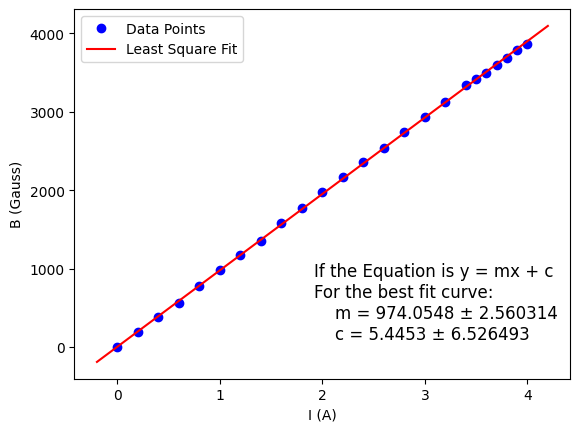
\includegraphics[width=0.8\columnwidth]{images/plot1.png}
        \caption{Magnetic field (B) vs Current (I) from the calilbration data fitted to a straight line}
        \label{plot:1}
    \end{figure}

    From this, $B$ for an arbitrary value of $I$ can be found as:

    \begin{equation}
        B = (974.0548\cdot I + 5.4453)\times10^{-4}\,T
    \end{equation}

    From Eq.(10), if we ignore the effects of $\chi_\text{air}$, we can write

    \begin{equation}
        h = \frac{\chi}{4g\mu_o(\rho - \rho_\text{air})}B^2
    \end{equation}

    Plotting $h$ vs. $B^2$, we get

    \begin{figure}[H]
        \centering
        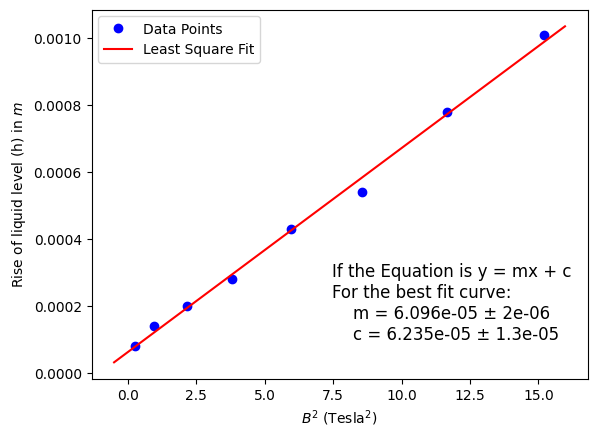
\includegraphics[width=0.8\columnwidth]{images/plot2.png}
        \caption{$h$ vs $B^2$ plot}
        \label{plot:2}
    \end{figure}

    where the slope is $m=6.096\times10^{-5}$. Rearranging Eq.(12), 
    \begin{equation*}
        \chi = m\cdot4g\mu_o(\rho - \rho_\text{air})
    \end{equation*}

    Using $g=9.81\,m/s^2$, $\mu_o=4\pi\cross10^{-7}\,H/m$, $\rho=1293.2\,kg/m^3$, $\rho_\text{air}=1.29\,kg/m^3$, we get

    \begin{align*}
        \chi = 3.88 \times 10^{-5} &= \chi_\text{Fe} + \chi_\text{water}\\
        \text{taking }\chi_\text{water}&=-9.04\times10^{-6},\\\
        \chi_\text{Fe} &= 4.79\times10^{-5}
    \end{align*}

    is the volume susceptibility of $\text{Fe}^{3+}$ solution. The mass susceptibility can be found by,

    \begin{align*}
        \chi'_\text{Fe} = \chi_\text{Fe}/\rho = 3.70\times10^{-8}\,m^2/kg
    \end{align*}

    Since $M = 0.169$ kg/mol, the molar susceptibility is,

    \begin{align*}
        \chi''_\text{Fe} = \chi'_\text{Fe}\times M = 0.63\times10^{-8}\,m^3/mol
    \end{align*}

    The Curie constant can be calculated as

    \begin{align*}
        C &= \chi''_\text{Fe}T,\,\,\, T=299K \\
        \implies C &= 1.89\times10^{-6}\,m^3 K/mol
    \end{align*}

    And magnetic moment ($\mu$) of the dipole of the specimen,

    \begin{align*}
       \mu = 2.8241\sqrt{C} = 3.89\times10^{-3}\,A/m^2
    \end{align*}


